\documentclass[a4paper,11pt]{article}

\usepackage[T1]{fontenc}
\usepackage{geometry}
\usepackage[protrusion=true,expansion=true]{microtype}
\usepackage[compact]{titlesec}
\usepackage{amsmath,amssymb}
\usepackage{mathtools}
\usepackage{fancyvrb}
\usepackage[font=small,labelfont=bf]{caption}
\usepackage{graphicx}
\usepackage{numprint}

\setlength{\parindent}{0in}
\setlength{\parskip}{1ex plus 0.5ex minus 0.2ex}

\begin{document}

\begin{figure}
\begin{center}
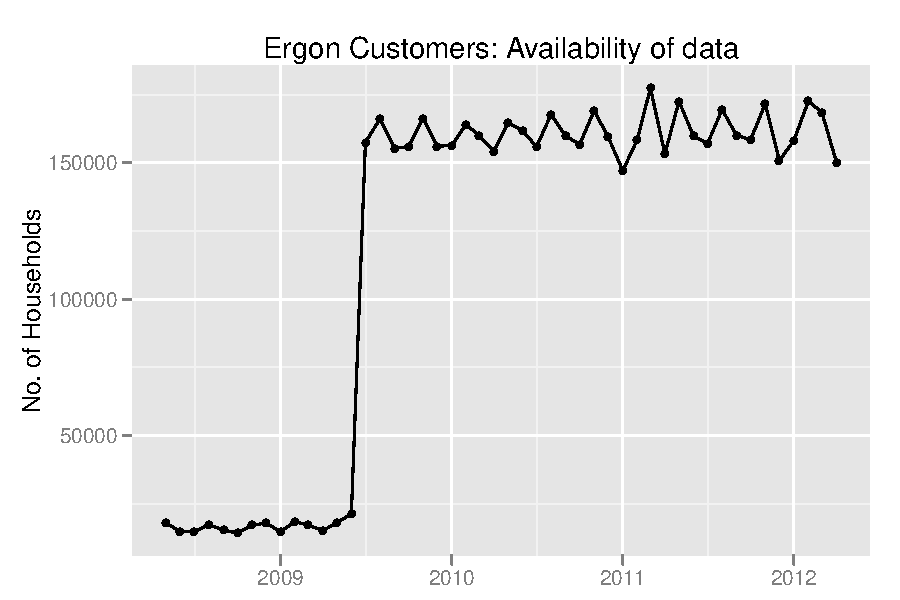
\includegraphics[width=1\textwidth]{figures/ErgonAvailData.pdf}
\caption{Have not filled in the space between bills. This is a count of
non missing values in the month.}
\end{center}
\end{figure}

\begin{figure}
\begin{center}
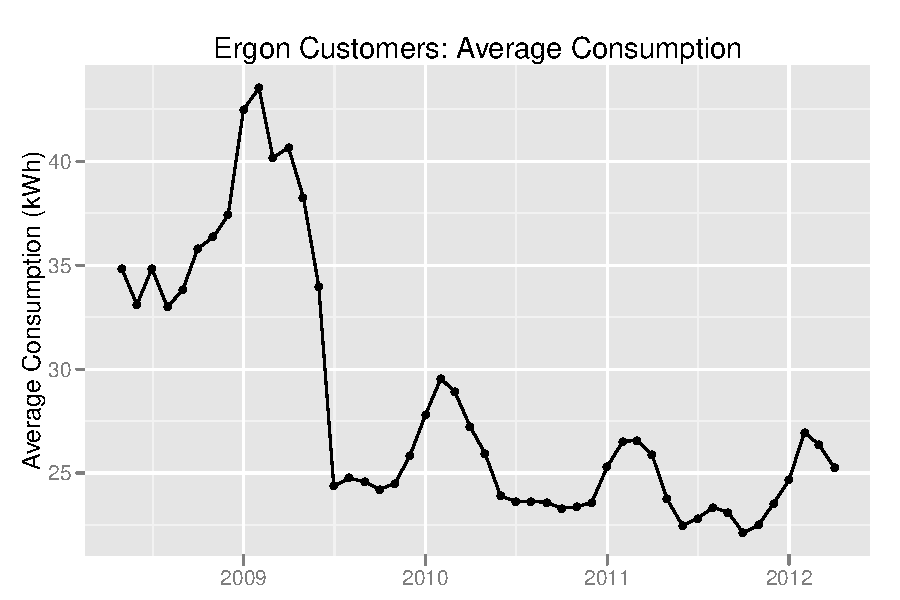
\includegraphics[width=1\textwidth]{figures/ErgonAvgConsump.pdf}
\caption{The average of non-missing values in the month.}
\end{center}
\end{figure}

\begin{figure}
\begin{center}
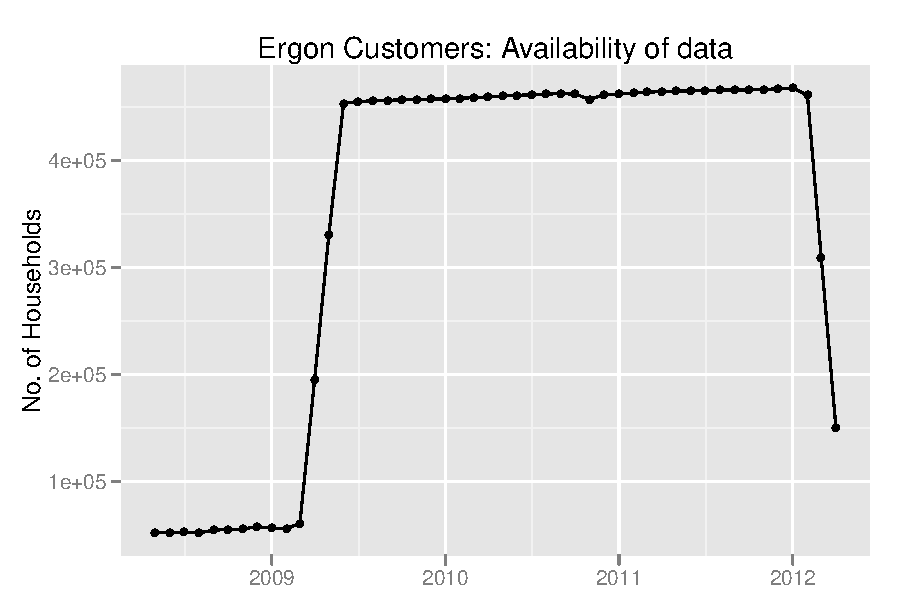
\includegraphics[width=1\textwidth]{figures/ErgonAvailDataFilled.pdf}
\caption{Filled with values up to 3 periods away to the right. This is a
count of non missing values in the month.}
\end{center}
\end{figure}

\begin{figure}
\begin{center}
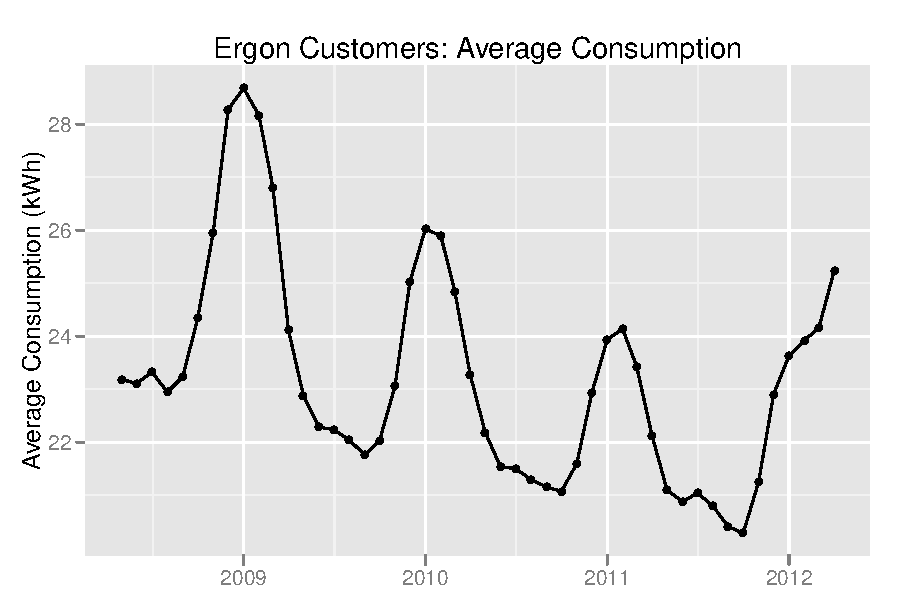
\includegraphics[width=1\textwidth]{figures/ErgonAvgConsumpFilled.pdf}
\caption{Filled with values up to 3 periods away to the right. The average
of non-missing values in the month.}
\end{center}
\end{figure}

\begin{figure}
\begin{center}
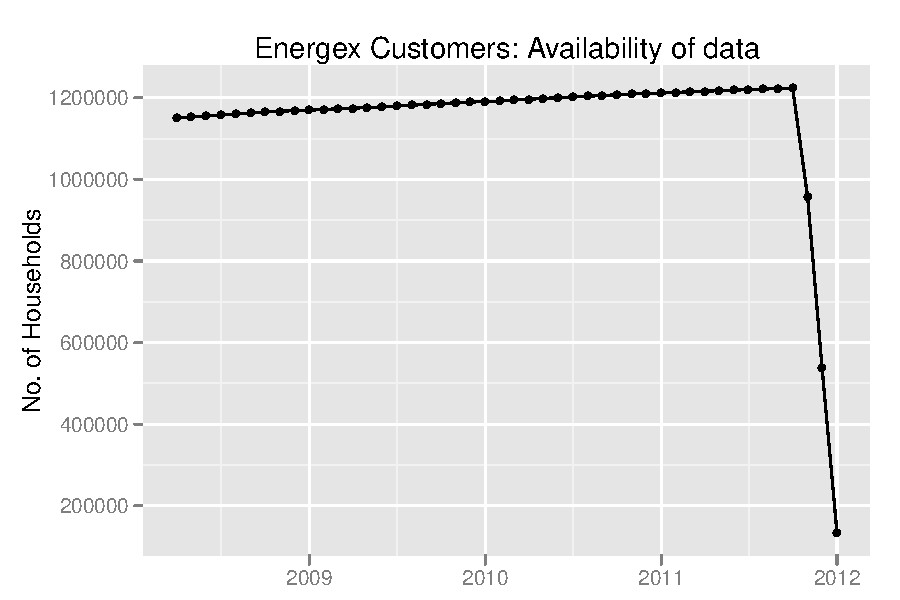
\includegraphics[width=1\textwidth]{figures/EnergexAvailData.pdf}
\caption{The number of unique households for which there is data (i.e.
where {\tt P\_MONTH\_*} is not zero.)}
\end{center}
\end{figure}

\begin{figure}
\begin{center}
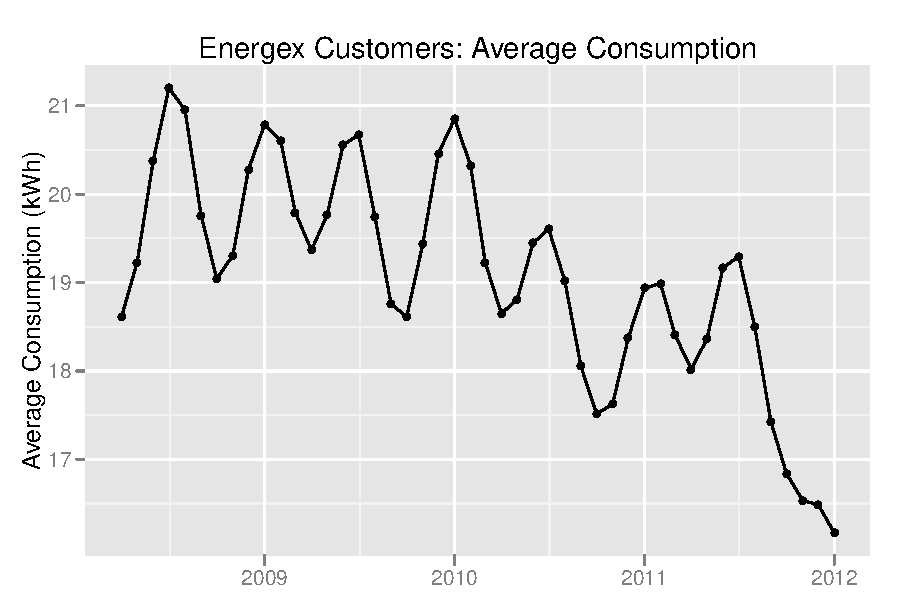
\includegraphics[width=1\textwidth]{figures/EnergexAvgConsump.pdf}
\caption{For consumption values where {\tt P\_MONTH\_*} is non zero,
consumption is scaled as {\tt CONS\_X/P\_MONTH\_X}. Household consumption
sum across tariff type in each period and plotted is the average across
households by period.}
\end{center}
\end{figure}

\begin{figure}
\begin{center}
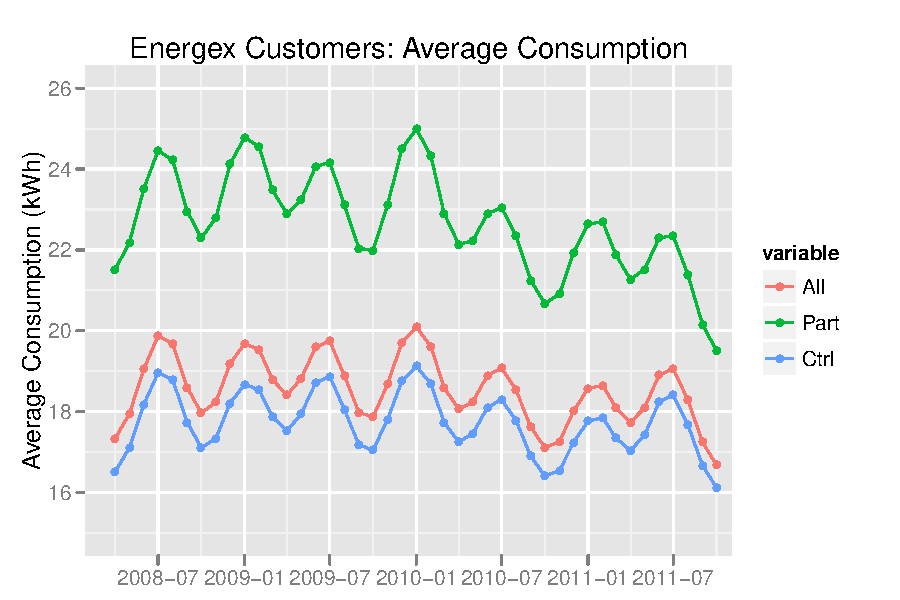
\includegraphics[width=1\textwidth]{figures/EnergexAvgConsump1.pdf}
\caption{Participants are households who end up joining the program.}
\end{center}
\end{figure}

\begin{figure}
\begin{center}
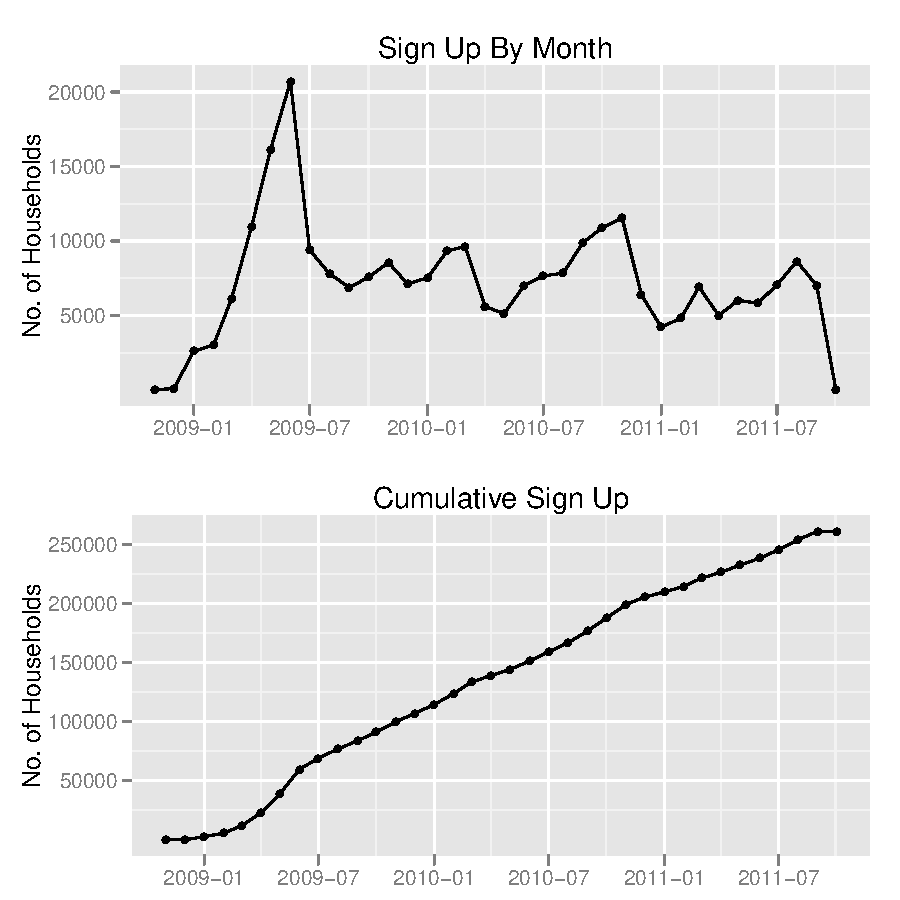
\includegraphics[width=1\textwidth]{figures/PartSignUp.pdf}
\caption{Program sign up.}
\end{center}
\end{figure}

\begin{figure}
\begin{center}
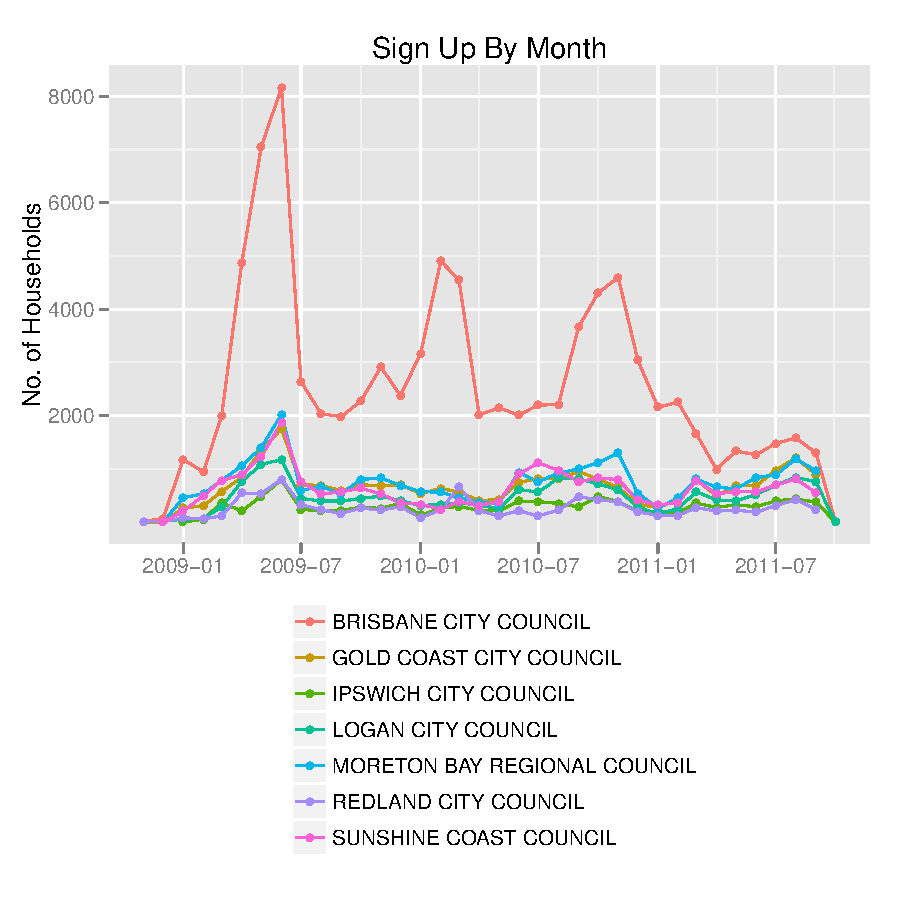
\includegraphics[width=1\textwidth]{figures/PartSignUpByLga1.pdf}
\caption{Program sign up by the seven LGA with the most participants.}
\end{center}
\end{figure}
\begin{figure}
\begin{center}
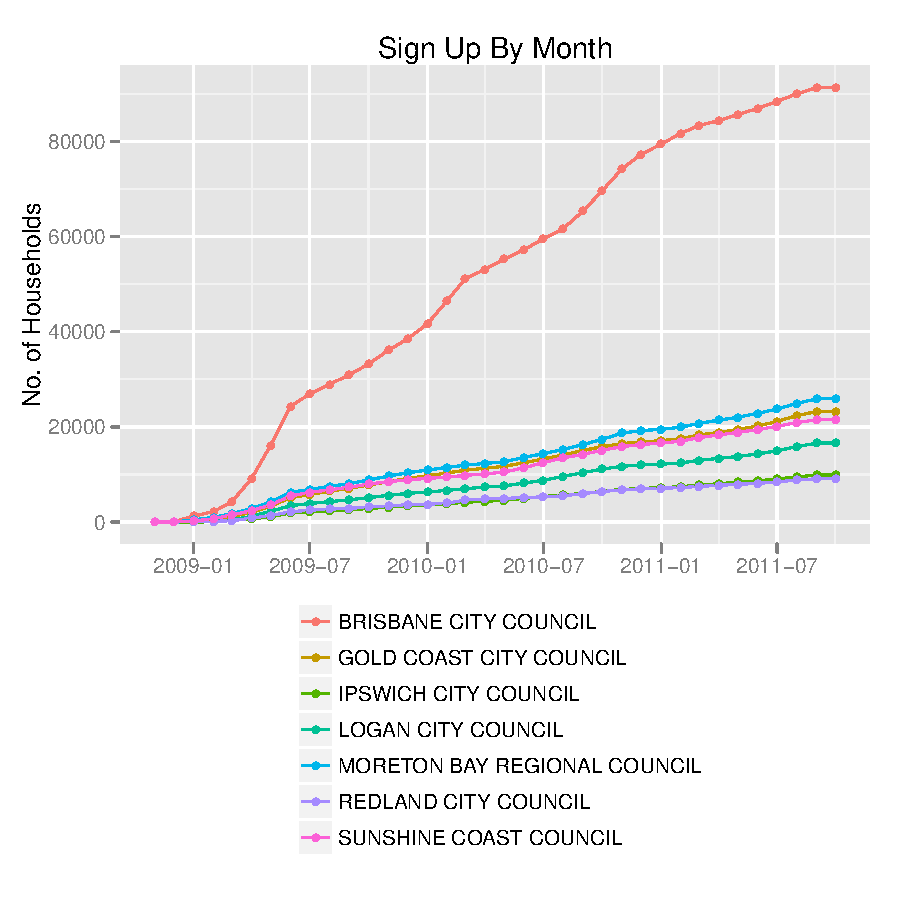
\includegraphics[width=1\textwidth]{figures/PartSignUpByLga2.pdf}
\caption{Program sign up by the seven LGA with the most participants.}
\end{center}
\end{figure}

\begin{figure}
\begin{center}
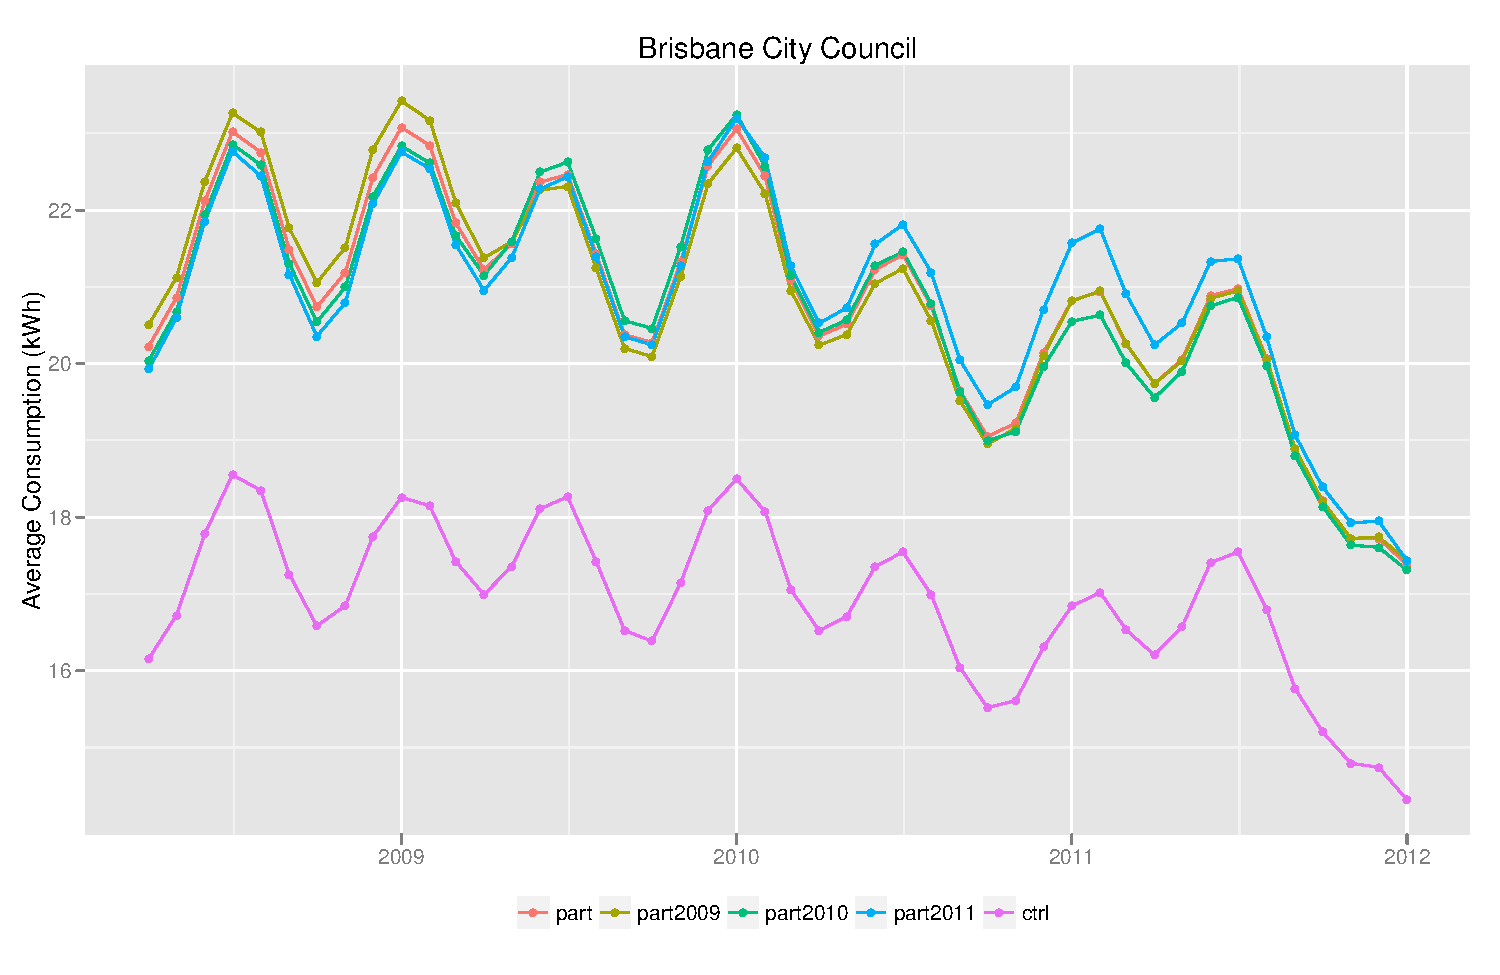
\includegraphics[width=1\textwidth]{figures/BrisbaneConsump.pdf}
\caption{Consumption of participant is additionally broken down into the
year households entered the program, e.g. part2009 shows the average
consumption of households (\numprint{38424} in all) who joined the program
in 2009. [2010: \numprint{38806}; 2011: \numprint{14020}; and 2008: 81
(not shown)]}
\end{center}
\end{figure}

\begin{figure}
\begin{center}
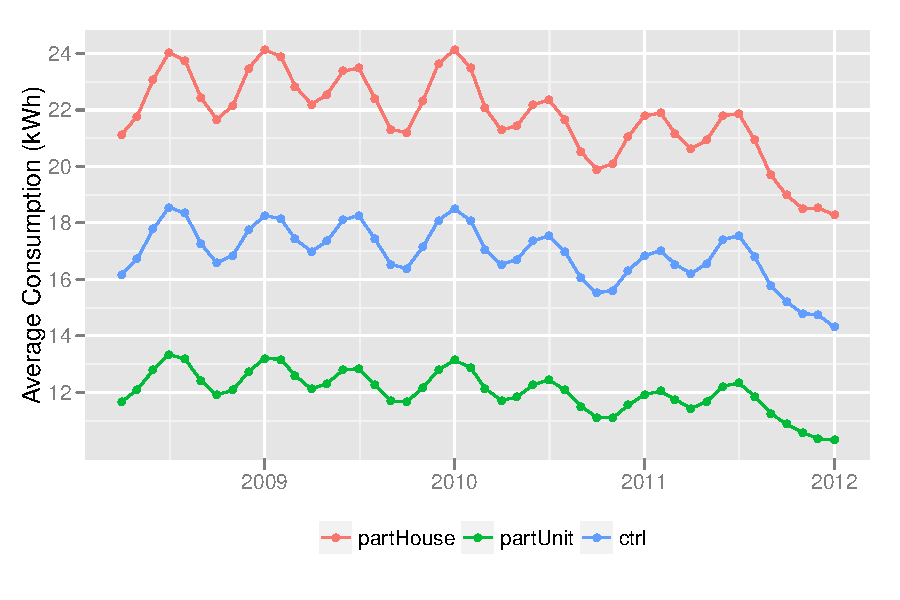
\includegraphics[width=1\textwidth]{figures/BrisHouseUnit.pdf}
\caption{Consumption of Brisbane participants grouped by whether the
household dwelling is a house or unit/apartment. Of \numprint{91331}
Brisbane participants 88.7\% (\numprint{81040}) live in houses.}
\end{center}
\end{figure}

\begin{figure}
\begin{center}
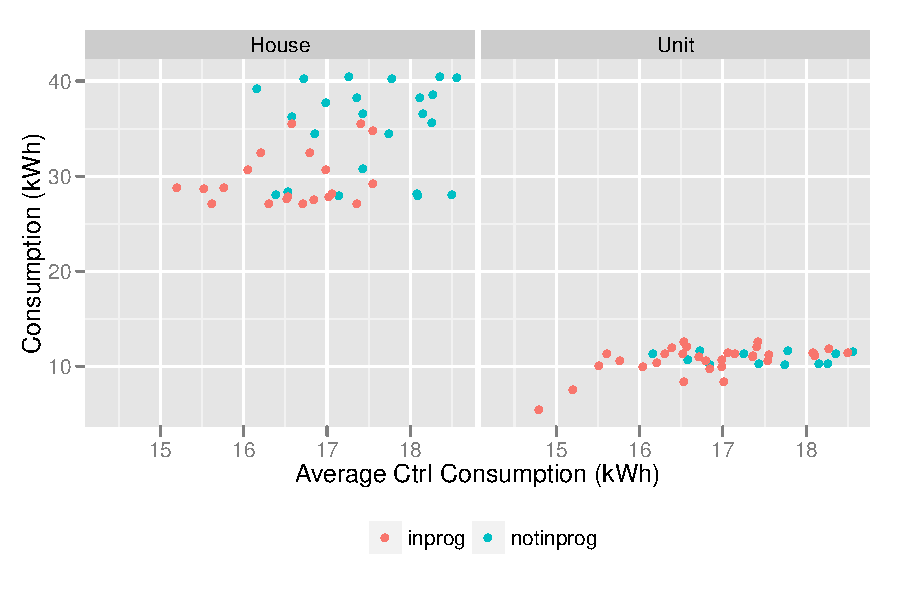
\includegraphics[width=1\textwidth]{figures/BrisSamp1.pdf}
\caption{Comparing the consumption of two Brisbane households against the
average of the control consumption (i.e. Energex customers in Brisbane not
in the program) before and after they enter the program.}
\end{center}
\end{figure}

\begin{figure}
\begin{center}
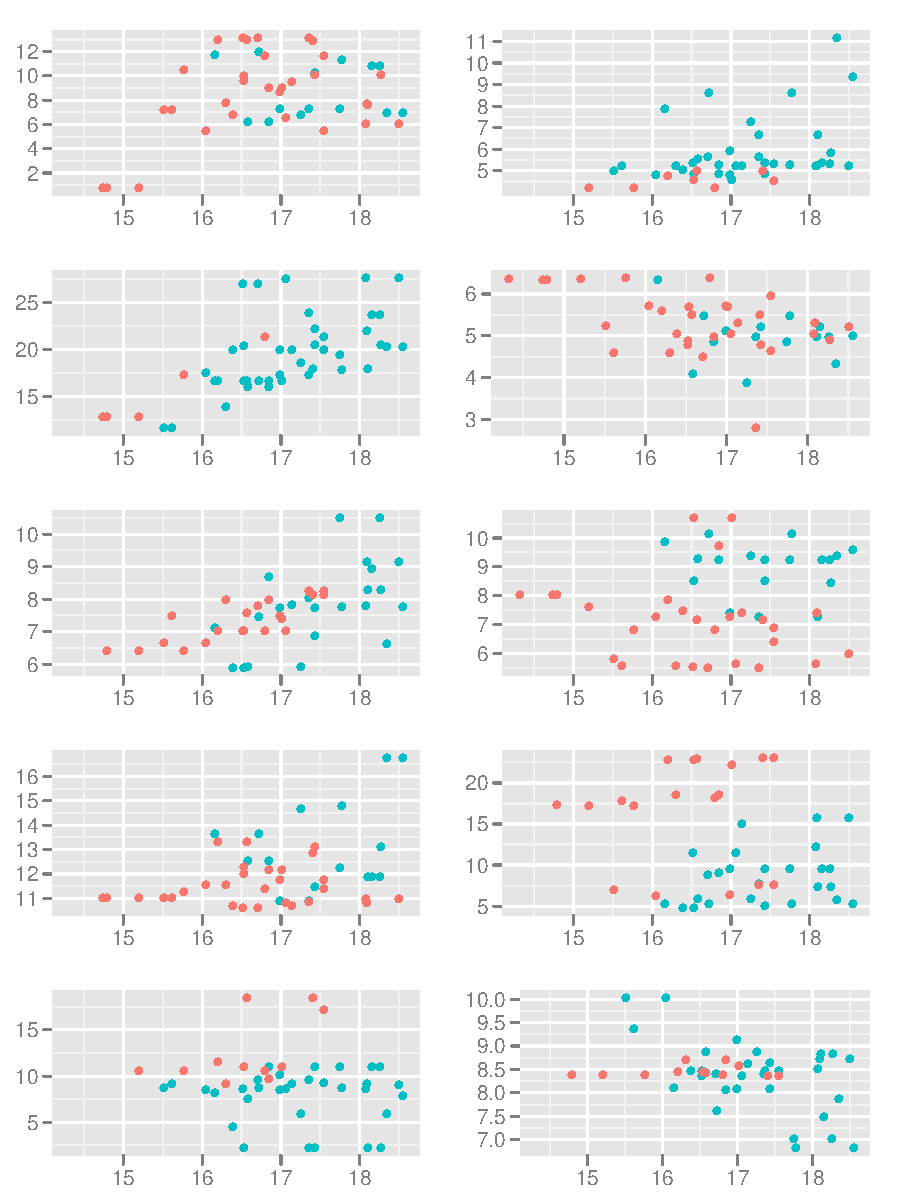
\includegraphics[width=1\textwidth]{figures/BrisSamp2.pdf}
\caption{More households: the left column remains those living in houses,
while the right are those living in units or apartments.}
\end{center}
\end{figure}

\end{document}


